%%%%%%%%% PROJECT DESCRIPTION  -- 15 pages (including Prior NSF Support)

\required{Project Description}
\begin{center}
%\emph{Maximum of 15 pages}
\end{center}
%The Project Description (including Results from Prior NSF Support, which is
%limited to five pages) may not exceed 15 pages. Visual materials, including charts,
%graphs, maps, photographs and other pictorial presentations are included in the
%15-page limitation. PIs be cautioned that the project description must
%be self-contained and that URLs that provide information related to the proposal
%should not be used. \\
%
%All proposals to NSF are reviewed utilizing the two merit review criteria,
%intellectual merit and broader impacts. \\
%
% The Project Description should provide a clear statement of the work 
% to be undertaken and must include: objectives for the period of the proposed 
% work and expected significance; relation to longer-term goals of the PI's 
% project; and relation to the present state of knowledge in the field, 
% to work in progress by the PI under other support and to work in progress 
% elsewhere.

%%%%%%%%%%%%%%%%%%%%%%%%%%%%%%%%%%%%%%%%%%%%%%%%%%%%%%%%%%%%%%%%%%%%%%
%INTRO
%%%%%%%%%%%%%%%%%%%%%%%%%%%%%%%%%%%%%%%%%%%%%%%%%%%%%%%%%%%%%%%%%%%%%%
\section*{Introduction}

Due to their sessile nature, natural selection will act to adapt plants to their local environments \citep{stebbins1950variation}. Understanding the genetic basis of how plants adapt to local conditions -- how many loci are involved, what are their effect sizes, and how similar are they among populations and species -- will thus allow for improved breeding and conservation strategies.  This is particularly pressing given current issues of climate change, habitat loss, and population growth.  These pressures will require adaptation of crops and wild plants to changing local conditions and cultivation of crops in new locales to meet growing demand.   
%Do we need citations here? Not sure %Kawecki2004 and \citep{savolainen2013ecological} still appropriate.

Agricultural species represent  promising systems for ongoing research on local adaptation.  Most crops were domesticated in narrow geographic centers but encountered and adapted to a wide range of novel environments as agriculture expanded across the globe.  In many instances  traits important for  local adaptation have already been identified.  These systems therefore represent compelling opportunities for investigating the genetic architecture of local adaption.  Moreover, insights gained regarding adaptive loci can feed back into modern crop improvement, yielding valuable benefits in the face of  rapid environmental change.
%do we need citations here?

{\bf Here we propose to use maize adaptation (\emph{Zea mays} ssp. \emph{mays}) to high elevation environments as a model for understanding the genetic basis of local adaptation in plants}.  Maize was domesticated in the lowlands of southwest Mexico from the narrowly distributed teosinte \emph{Zea mays} ssp. \emph{parviglumis} \citep[hereafter, \emph{parviglumis};][]{Matsuoka2002}. Since domestication, maize has spread worldwide: analysis of cultivation area data  indicates maize has the greatest global geographic breadth of 16 staple crops (Figure \ref{fig:breadth}) and is now cultivated on six continents, ranging from southern Chile to Canada \citep{tenaillon2011european} and from sea level to well over 3000m in altitude. In addition to maize and \emph{parviglumis}, a related  teosinte \emph{Zea mays} ssp. \emph{mexicana} (hereafter, \emph{mexicana}) is found only in highland environments, having adapted to highland environments thousands of years prior to maize domestication \citep{Ross-Ibarra2009a, hufford2012inferences}. Maize and teosinte thus form an ideal system in which multiple replicated evolutionary experiments will allow us to dissect the genetic architecture of highland adaptation as a model for understanding plant local adaptation.

\begin{SCfigure}[][h]
  \centering
  \caption{Geographic breadth of the world's 16 staple crops, expressed in percent of land surface area in which each crop is cultivated. Data are from \citet{monfreda2008farming}. } 
   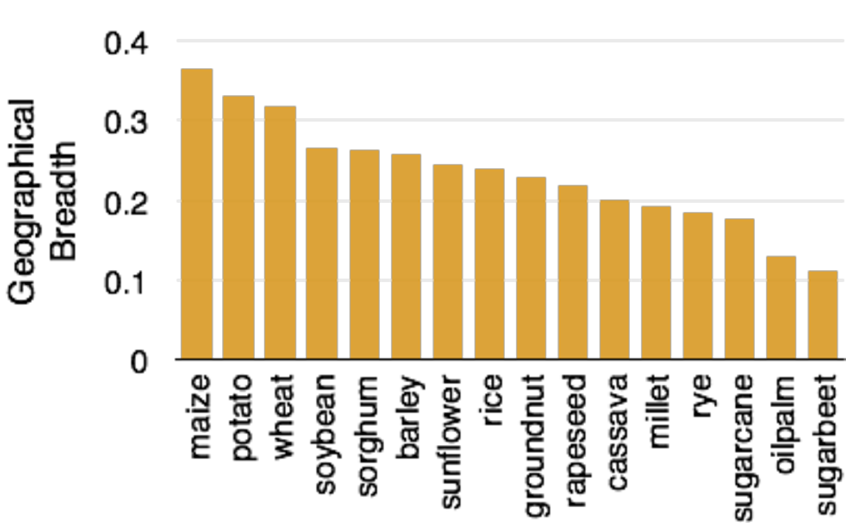
\includegraphics[width=0.5\textwidth]{breadth.png}
\label{fig:breadth}
\end{SCfigure}

%%%%%%%%%%%%%%%%%%%%%%%%%%%%%%%%%%%%%%%%%%%%%%%%%%%%%%%%%%%%%%%%%%%%%%
%AIMS
%%%%%%%%%%%%%%%%%%%%%%%%%%%%%%%%%%%%%%%%%%%%%%%%%%%%%%%%%%%%%%%%%%%%%%
\section*{Aims}

We will investigate the genetic basis of highland adaptation in maize by achieving three aims:

\begin{enumerate}
\item {\bf Dissect the genetic architecture of highland traits}
\item {\bf Investigate population genetic signatures of highland adaptation}
\item {\bf Characterize functional variation at adaptive quantitative trait loci}
\end{enumerate}

%%%%%%%%%%%%%%%%%%%%%%%%%%%%%%%%%%%%%%%%%%%%%%%%%%%%%%%%%%%%%%%%%%%%%%
%RATIONALE AND SIGNIFICANCE
%%%%%%%%%%%%%%%%%%%%%%%%%%%%%%%%%%%%%%%%%%%%%%%%%%%%%%%%%%%%%%%%%%%%%%
\section*{Rationale and Significance}

While the genetic basis of local adaptation is generally not well understood, the declining cost of genotyping has enabled a handful of genome-wide studies across populations of model species.  For example, \citet{fournier2011map} demonstrated that alleles associated with high fitness in \emph{Arabidopsis thaliana} have a tendency to be both local and linked to climate.  Likewise, a recent study across hundreds of accessions of \emph{Medicago truncatula} identified candidate loci for local adaptation and found them to be predictive of growth rate under temperature and soil moisture treatments \citep{Yoder17012014}.  Finally, our own genome-wide study of teosinte (the wild relatives of maize) revealed  an important role for inversion polymorphisms and -- in contrast to results from \emph{Arabidopsis} \citep{hancock2011adaptation} -- an enrichment of regulatory variants among loci showing evidence of selection \citep{Pyhajarvi2013}. While much of local adaptation may involve complex quantitative traits \citep{le2012genetic}, the genetic architecture of these traits does not necessarily mirror results from mapping studies in other populations. In maize, for example, although genome-wide association in the NAM panel suggests that flowering time is largely controlled by many loci of small effect \citep{buckler2009genetic}, adaptive change in flowering time across latitudes has involved loci of large effect on photoperiod \citep{hung2012zmcct}. The strength and timing of selection on a trait also plays a role: while ear and tassel traits in maize share a number of QTL, those underlying ear morphology, which underwent recent strong selection during domestication, are of larger mean effect size \citep{Brown2011b}. Though initial genomic studies are beginning to yield valuable insights regarding local adaptation, clearly much remains to be discovered.  

Highland adaptation in maize and teosinte are an excellent system in which to study local adaptation.  Following domestication, maize spread to the highlands of the Central Plateau, a migration across more than 1000m of increasing elevation.  Colonization of the highlands required adaptation to a number of novel abiotic conditions, including gradients of temperature, precipitation, and elevation. Highland landraces have distinct morphologies (e.g., highly pigmented and hairy leaves and stems) that are believed to confer adaptation to this cooler region \citep{Doebley1984a}.  Our previous genetic analyses \citep{vanheerwaarden2011a} show that maize has independently adapted to highland environments multiple times, including the southwest US and the Andes of South America, where landraces (i.e., local farmer varieties) are commonly grown above 3000m. Multiple independent instances of highland adaptation in maize and teosinte provide replicated evolutionary experiments, providing power to identify and validate loci common candidate loci as well as discover multiple potential mechanisms for highland adaptation unique to each population.

Study of the genetic architecture of maize adaptation will provide both basic evolutionary insight and essential information to help increase or sustain yield in the face of human population growth and climate change. Historical analyses suggest that climate change over the last 30 years has already dramatically impacted maize yields worldwide, slowing gains from breeding and management \citep{Lobell2011}.  \citet{Lobell2011b} further determined that future temperature increases will likely decrease yield across 65\% of African maize-growing regions, while all of Africa  will see diminished maize yield if increased temperature is accompanied by drought.  An understanding of how maize has adapted to challenging environmental conditions in the past will help breeders to mitigate yield loss due to future changes.

%Do we need more text on why anyone should care about local adaptation to begin with? How it's relevant for breeding?

%check out these for ev. that traits are adaptive, cited in Lauter 2004:
%Lauter, N., 2001 The inheritance and evolution of quantitative traits in teosinte. Ph.D. Dissertation, University of Minnesota, St. Paul.
%Doebley 1984 paper cited above.

%%%%%%%%%%%%%%%%%%%%%%%%%%%%%%%%%%%%%%%%%%%%%%%%%%%%%%%%%%%%%%%%%%%%%%
%PRELIMINARY RESULTS
%%%%%%%%%%%%%%%%%%%%%%%%%%%%%%%%%%%%%%%%%%%%%%%%%%%%%%%%%%%%%%%%%%%%%%
\section*{Preliminary Results}
Preliminary work from project members positions us to make excellent progress on our proposed aims. Co-PIs Ross-Ibarra and Hufford have worked extensively on the population genetics of highland adaptation.    \citet{Pyhajarvi2013} explored local adaptation in \emph{parviglumis} and \emph{mexicana} populations, finding a large number of loci showing association with altitude and evidence of selection, as well as highlighting the potential importance of regulatory variants and large inversion polymorphisms. This study identified a putatively adaptive inversion on chromosome four that distinguishes the lowland \emph{parviglumis} from the highland \emph{mexicana} and coincides with a quantitative trait locus associated with  traits  linked to highland adaptation \citep{Lauter2004a}. This \emph{Inv4m} inversion is the subject of our functional characterization in \ref{sec:funchar}.  \citet{Pyhajarvi2013} also identified populations of \emph{parviglumis} showing extensive admixture with the highland \emph{mexicana} which are the subject of proposed analysis in \ref{subsec:admixmap,sec:admixpopgen}. \citet{Hufford2013} identified genomic regions in highland maize that have introgressed from the highland  \emph{mexicana}.  They showed that  plants with \emph{mexicana} alleles showed highland phenotypes and superior growth under cold conditions, suggesting an adaptive role for introgression and motivating our population genetic analyses in \ref{sec:selection}.  Finally, recent analyses of selection in genotyping data from a wide collection of landraces from the highlands of Mexico and S. America finds little overlap in the genes important for adaptation (Takuno \emph{et al.} In Prep; Figure \ref{fig:fst}), motivating the QTL analysis in \ref{sec:qtlmap}.

\begin{SCfigure}[][t]
  \centering \label{fig:fst}
   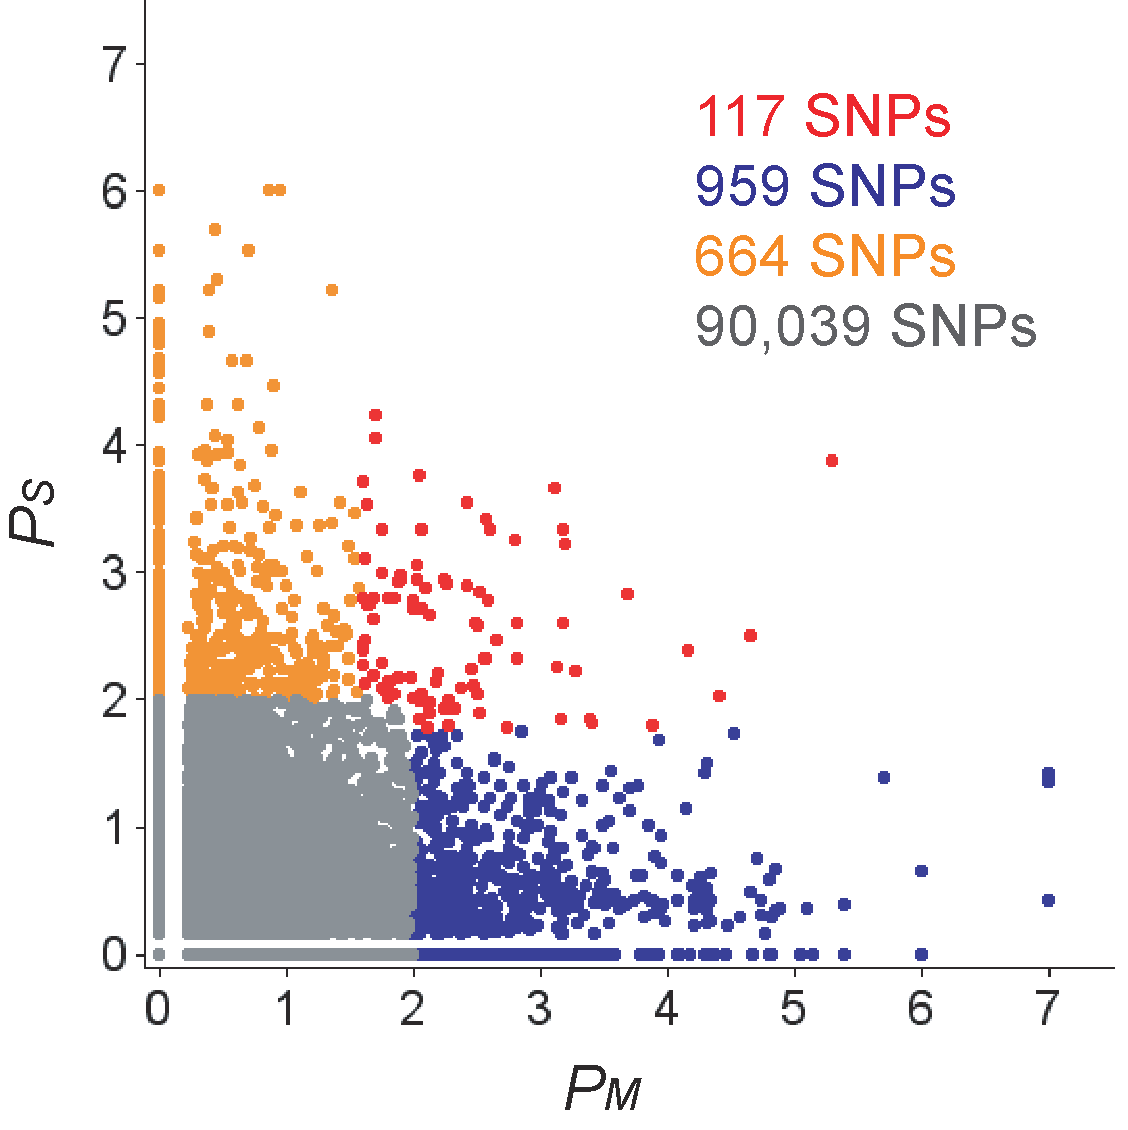
\includegraphics[width=0.4\textwidth]{fst.pdf}
  \caption{Little overlap of adaptive loci between continents. Shown is a scatter plot of $-log_{10}$ empirical p-values of genetic differentiation ($F_{ST}$) in Mexico ($P_M$ on $x$-axis) and S. America ($P_S$ on $y$-axis).  SNPs showing evidence of selection are highlighted in blue (Mexico), orange (S. America), or red (both Mexico and S. America), along with the number of SNPs in each category.} 
\end{SCfigure}

Co-Pi Flint-Garcia and Sr. Personnel Sawers have made important progress on the development of populations for the project. For \ref{subsec:qtlmap} our Mexican  cross is already at the F2 generation, and one potential S. American cross is now at the F1 generation  (Table \ref{tab:qtlpops}).  Back-crosses of the reference genome inbred B73 to a highland Mexican landrace Palomero Toloque\~no have been made and selfed to generate a BC1S1 population that will be further developed in \ref{subsec:nils} to dissect the function of the \emph{Inv4m} polymorphism. Both SSRs and SNPs that distinguish the  \emph{mexicana} alleles at \emph{Inv4m} have also been developed.

Co-PI Coop has worked to develop analytical approaches to understanding local adaptation, including methods that allow genome-wide association with environmental variables \citep{Coop2010, gunther2013robust}, detection of selection in introgressed populations \citep{Brandvain2013}, and powerful approaches to identify phenotypic selection on quantitative traits \cite{Berg2013}.  His group is currently working on methods for mapping and studying adaptation in admixed populations.
%!HELP add Torsten's citation

%%%%%%%%%%%%%%%%%%%%%%%%%%%%%%%%%%%%%%%%%%%%%%%%%%%%%%%%%%%%%%%%%%%%%%
%SPECIFIC OBJECTIVES
%%%%%%%%%%%%%%%%%%%%%%%%%%%%%%%%%%%%%%%%%%%%%%%%%%%%%%%%%%%%%%%%%%%%%%
\section*{Specific Objectives}

%%%%%%%%%%%%%%%%%%%%%%%%%%%%%%%%%%%%%%%%%%%%%%%%%%%%%%%%%%%%%%%%%%%%%%
%AIM 1
%%%%%%%%%%%%%%%%%%%%%%%%%%%%%%%%%%%%%%%%%%%%%%%%%%%%%%%%%%%%%%%%%%%%%%

\renewcommand{\thesection}{Aim \arabic{section}}
\section{Genetic architecture of highland traits} \label{sec:qtl}

One of the primary goals of this proposal is to determine the genetic architecture of highland adaptation. Ultimately, this knowledge will be useful for determining the genes underlying these loci (\ref{sec:funchar}) and the pathways involved in adaptation (\ref{sec:selection}). These loci can also be used in maize improvement via marker assisted selection. In this aim we wish to determine how many genomic regions control adaptive phenotypes, where these regions are located, and the distribution of allelic effects at these loci. We first perform comparative QTL analysis in two highland x lowland crosses (\ref{subsec:qtlmap}), then take advantage of historical recombination and greater resolution to map loci in an admixed population of highland and lowland teosinte (\ref{subsec:admixmap}).

\subsection*{Questions}
\begin{itemize}[topsep=0pt,itemsep=-1ex,partopsep=1ex,parsep=1ex]
\item What is the genetic architecture of highland adaptation?
\item How much of the genetic architecture is shared between Mexico and South America?
\item How much of the genetic architecture is shared between maize and teosinte?
\end{itemize}

\subsection{QTL mapping of highland adaptation} \label{subsec:qtlmap}

Our first objective is to identify  genomic regions controlling highland adaptation in maize.  We will conduct QTL mapping studies of one Mexican and one South American population, each derived by crossing a landrace adapted to lowland conditions with a  landrace adapted to highland conditions (Table \ref{tab:qtlpops}).  We make use of specially-inbred landrace lines created by John Doebley (U. Wisconsin) and Seth Murray (Texas A\&M), thus simplifying downstream applications and allowing replication of alleles in our functional studies (see \ref{sec:funchar}). 

\begin{table}
\begin{center}
\caption{Parental lines for QTL} \label{tab:qtlpops}
\begin{tabular}{llll}\\\toprule  
{\bf Population}	& {\bf Parent } &	{\bf Origin (masl)} & {\bf Status }\\ \midrule
 \rowcolor{gray!25}
Mexico	& Zapalote Chico		& Oaxaca	 (46)		&  F2 \\ 
 \rowcolor{gray!25}
	& 	Palomero de Jalisco	& 	Jalisco (2520)		& \\
S. America	& Araguito	& Venezuela (183)	&  F1 \\ 
	& Sal Prieta	 & Ecuador (2948) & \\ \bottomrule
\end{tabular}
\end{center}
\end{table} 

We will self-pollinate the F2 plants to create 500 F2:3 families from each population.  DNA will be extracted from each of the F2 plants and sequenced to 20-30X depth on two lanes of Illumina (150bp paired-end reads on a HiSeq 2500 at the UC Davis Genome Center), providing genome-scale SNP data similar to our previous work \citep[HapMap.v2;][]{Chia2012a}.  F2 plants will be genotyped using genotyping-by-sequencing \citep[GBS;][]{Elshire2011} and run through the standard maize GBS pipeline \citep{Glaubitz2014} resulting in approximately \textasciitilde 1M SNPs, allowing straightforward imputation of their full-genome sequence.  The genetic map will be created using standard methods \citep[e.g.][]{Broman2003a}. 

Populations will be phenotyped at 3 field locations, including one lowland site (Valle de Banderas in Mexico), one highland site (Irapuato or Queretaro, Mexico), and one temperate site near Columbia, Missouri (Table \ref{tab:locales}).  At each field location, best local practices will be used including fertilizers and pest and weed control.

\begin{table}
\rowcolors{2}{gray!25}{white}
\begin{center}
\caption{Common garden locations} \label{tab:locales}
\begin{tabular}{p{2cm}cccccc}\\\toprule  
{\bf Field Sites} & {\bf Lat/Lon } & {\bf Elevation\,(m) } &	{\bf Min/Mean/Max\,$^{\circ}\mathrm{C}$  } & {\bf Precip\,(mm) } \\ \toprule
Valle de Banderas, Nayarit	& 20.8,\,-105.2&	54		&	15.3/25.8/33.7	&	1184 \\
Irapuato, Guanajuato 	&	20.7,\,-101.3	&	1729.0	&	7.3/20.2/31.7	&	693 \\
Amealco, Quer\'etaro 	&	19.5,\,-99.1	&	2240.0 	&	2.3/15.6/27.0	&	626\\
Columbia, Missouri		& 	28.9,\,-92.2	&	266.1 	&	-17.8/36.0/40.5&	914\\ \bottomrule
\end{tabular}
\end{center}
\end{table} 

At each site, the experiment will consist of two replicates in which the 500 entries  will be arranged in an augmented alpha lattice design.  Parental checks will be included to control for field variation.  We will collect a  number of phenotypes (Figure \ref{fig:phenos}) using our in-house barcode-based data collection program. Germination assays  in controlled conditions will be conducted in Ames, Iowa, and root chilling will be evaluated using a custom hydroponic system at the University of California, Davis (see letter of support from Dr. Arnold Bloom).    

\begin{figure}[ht!]
	\begin{minipage}{0.5\textwidth}
    		\centering
   		\includegraphics[width=\textwidth]{fourtraits.pdf}
  	\end{minipage}%
  	\begin{minipage}[c]{0.50\textwidth}
  		\centering
		\rowcolors{2}{gray!25}{white}
		\begin{tabular}{llcc}\\\toprule  
		{\bf Trait} & {\bf Phenotype}  \\\midrule
		MH & leaf sheath macrohairs  \\
		DTS & days to silking  \\
		DTA & days to anthesis  \\
		PH & plant height 			\\
		BM & total plant biomass 	\\
		EH & ear height			 \\
		EN & ear number			 \\
		FK & fifty kernel weight \\
		TN & tassel number \\
		TBN & tassel branch number \\
		TL & tassel length \\
		SM & total kernel mass \\
		RC & root chilling response \\
		GDP & germination depth \\
		SC & stem anthocyanin content \\
		GDP & germination depth \\
		GDT & germination temperature \\\bottomrule
		\end{tabular}
	\end{minipage}
 	\caption{ Phenotypic differences between a sampling of highland and lowland landraces from Mexico and S. America, grown in common garden in Puerto Rico (left). List of the phenotypes to be measured in the field (right) }%
	\label{fig:phenos}
\end{figure}

Raw data from each plot will be analyzed using mixed-models incorporating replications and environments.  Data will be analyzed across environments to determine whether location (elevation) affects the various phenotypes.  Each location will then be analyzed separately to derive least squares means to be used as  phenotypic data in QTL analyses.  QTL analysis will be conducted using standard software (e.g. SAS; R/qtl \citealp{Broman2003a}).  Several iterations of QTL analysis will be conducted: on individual traits, individual traits adjusted for covariates such as flowering time, and multiple traits simultaneously.   QTL profiles will be compared across populations (Mexico vs South America) and field sites (elevation) to determine differences in how elevation affects putatively adaptive traits.  Comparison of the genetic architecture among traits will inform us of the lability of these traits and their amenability to selection via breeding.  Finally, the contrast of each Mexican location to the Missouri location will account for daylength differences and agronomic value in the Midwest. 

The expected outcomes of this objective will be 1) A map of QTL underlying phenotypic differences between highland and lowland maize in Mexico and South America, detailing the number and effect size of each QTL and differences between crosses, and 2) Estimates of fitness differences (PH, BM, SM, and FK (Figure \ref{fig:phenos}) of highland and lowland plants, as well as F2 with various combinations of QTL, in both environments. 

\subsection{Admixture mapping in a teosinte hybrid zone} \label{subsec:admixmap}
While \emph{mexicana} and \emph{parviglumis} are largely allopatric, the subspecies overlap in two regions of Mexico, eastern Jalisco state and the eastern Balsas River Basin \citep{hufford2012inferences}, and a number of hybrid populations have been documented in these regions \citep{Fukunaga2005}.  We have previously documented near equal proportions of ancestry from the two subspecies   admixture in one of these populations near the town of Ahuacatitlan in the eastern Balsas \citep{Pyhajarvi2013}.  Growth chamber experiments also suggest plants in this population have higher fitness in cold conditions than other \emph{parviglumis} populations.  Moreover, the relatively short length of  haplotypes Ahuacatitlan shares with other  populations suggests that there has been extensive recombination since the initial admixture event, providing an ideal population for high-resolution admixture mapping of \emph{mexicana} highland adaptation traits.

In November of year one of the project we will travel to Ahuacatitlan and collect seed from 500 individuals drawn randomly from the population.  Seed samples will be transported to Langebio in Irapuato, Mexico for cold storage. A single seed per individual (500 total) will be germinated on filter paper and transplanted into our two Mexican field sites (Table \ref{tab:locales}).  Phenotypes detailed in Figure \ref{fig:phenos} will be collected for admixture mapping.  The majority of these traits are known to differ considerably between \emph{parviglumis} and \emph{mexicana} (CITE).  Leaflet samples will be collected from plants in the field at the seven-leaf stage, and extracted DNA will be genotyped using GBS.  Several computational methods for admixture mapping have already been developed (  \citet{winkler2010admixture}), but we will augment these with methods currently under development by Co-PI Coop.  

However, these methods are not well suited to admixture mapping when there are differentially related individuals in the sample, and when natural selection may have systematically distorted admixture at some loci. In natural admixed populations these issues can be expected to occur, and will potentially result in false positives due to the non-independence of individuals (a fact accounted for in plant GWAS, but not in admixture mapping). We will implement novel methods currently under development by Co-PI Coop in our analysis of the Ahuacatitlan population that incorporate this non-independence into admixture association tests, while accounting for uncertainly in admixture calls along the genome. 

 %!HELP: writing & citation for parv/mex traits.
% CITE Lauter thesis?

%%%%%%%%%%%%%%%%%%%%%%%%%%%%%%%%%%%%%%%%%%%%%%%%%%%%%%%%%%%%%%%%%%%%%%
%AIM 2
%%%%%%%%%%%%%%%%%%%%%%%%%%%%%%%%%%%%%%%%%%%%%%%%%%%%%%%%%%%%%%%%%%%%%%
\section{Adaptive value of highland alleles} \label{sec:selection}

In aim \ref{sec:qtl} we will map loci corresponding to traits differing between highland and lowland maize and teosinte. In this section we will test the adaptive significance of QTL identified in \ref{sec:qtl} in three natural introgression experiments: gene flow from \emph{mexicana} into highland maize \ref{subsec:intropopgen} and admixture between \emph{mexicana} and \emph{parvgilumis} \ref{subsec:admixpopgen}. 

\subsection*{Questions}
\begin{itemize}[topsep=0pt,itemsep=-1ex,partopsep=1ex,parsep=1ex]
\item Are highland QTL/loci widespread in highland climes?
\item Are loci controlling phenotypic differences between highland and lowland populations adaptive?
\item Does natural selection favor introgression from adapted populations?
\end{itemize}

\subsection{Global analysis of highland haplotypes} \label{subsec:global}

% !HELP: writing

%\begin{itemize}
%\item Occurrence of highland haplotypes/QTL/SNPs in global pops (MBH)
%\item 500 worldwide accessions GBS (MBH)
%\item Berg's approach to show selection on traits in multiple highland popualtions
%\end{itemize}

Full genome resequencing underway will increase the resolution of this study and expand its scope to include maize from the highlands of Guatemala and the Southwestern United States.

And though quantitative genetic theory suggests that adaptive phenotypic change may not correlate with strong evidence for selection on individual loci \citep{le2012genetic}, recently developed methods from Co-PI Coop \citep{Berg2013} provide a powerful statistical framework to identify coordinated shifts in allele frequencies at causative QTL (from \ref{sec:qtl} to look for weak selection on alleles underlying highly quantitative traits.  

\subsection{Population genetics of maize-teosinte introgression} \label{subsec:intropopgen}

Our previous work \citep{Hufford2013} we documented extensive introgression between \emph{mexicana} teosinte and highland maize landraces, demonstrating an overlap with teosinte QTL for macrohairs and stem pigmentation \citep{Lauter2004a}. Because of the relatively low-density genotyping used, however, we were limited to identifying large regions of ancient introgression present in most populations.  We were also unable to investigate evidence of selection for any of the introgressed regions.  Here we propose to revisit these populations with higher-density genotyping that will allow identification of ongoing gene flow in individual populations and ask whether introgressed regions have been targeted by natural selection.  

We propose to resample 18 individuals from each of the same 9 sympatric population pairs and two allopatric populations studied in \citet{Hufford2013}. Each individual will be genotyped by GBS  using greater than normal depth (48 plex) to improve genotyping heterozygous sites.  These data will provide \textasciitilde 1M SNPs across the genome (compared to 40K SNPs in \citet{Hufford2013}). We will use both haplotype \citep{price2009sensitive} and heterozygosity-based \citep{Geneva2014} methods to identify introgressed segments in individual populations.  Genomic regions showing evidence of introgression will be tested for selection using population genetic approaches which utilize evidence from the site frequency spectrum \citep{nielsen2005genomic} and haplotype structure \citep{voight2006map}.  Correlations between genetic differentiation and recombination will allow us to investigate selection against introgression \citep{Brandvain2013}, quantifying the "linkage drag" associated with introgression of potentially beneficial adaptive alleles.  Finally, we will again apply the approach of \citet{Berg2013} to evaluate selection on individual phenotypes across highland maize landrace populations.

The expected outcomes of this objective are 1) a fine-scale dissection of both ancient and ongoing introgression 2) identification of introgressed regions showing evidence of positive selection, identifying loci important for highland adaptation,  3) evidence for selection on specific phenotypic traits, 4) quantification of the potential "linkage drag" or evidence against introgression across other regions of the genome.

%GBS of 18 inds x 10 pops x 2 subspecies (mex \& maize) (JRI)
%384 at 48 plex * \$60 = \$23040

\subsection{Population genetics of hybridization in teosinte} \label{subsec:admixpopgen}

In this objective, we will capitalize on the long history of gene flow between \emph{mexicana} and \emph{parviglumis} \citep{Ross-Ibarra2009a} to identify loci that show evidence of selection in admixed populations. To complement the Ahuacatitlan population from \ref{subsec:admixmap}, we will sample four additional admixed populations.  We have already identified multiple admixed populations using small-scale SNP data from across the range of each taxon \citep{vanheerwaarden2011a}.  We will revisit each of these populations to sample seed, collecting 50 individuals per population.  Samples will be genotyped via high-coverage (48plex) GBS to ensure accurate identification of heterozygous sites. The extensive gene flow between these taxa should lead to signatures of admixture throughout the genomes \citep{Pyhajarvi2013}.  Population genetic theory predicts, however, that adaptive loci which have introgressed due to natural selection should show distinct signals of elevated admixture, and our preliminary simulation results bear our this prediction (Figure \ref{fig:yaniv}). We will use these patterns of admixture, as well as more classical signals of selection (see \ref{subsec:intropopgen}) to identify loci showing evidence of adaptive introgression in these admixed populations.  Replicated admix populations, combined with the high resolution afforded by recombination in teosinte, will allow us to distinguish variants selected in individual populations vs. those showing parallel evidence of selection (repeated evolution) across all populations.  Signatures of repeated evolution are indicative of standing genetic variation or multiple pathways (a larger mutational target) to achieve a similar phenotypic outcome \citep{Ralph2010a}. Finally, the large sample sizes used will also allow us to identify coordinated shifts in allele frequencies \citet{Berg2013} of even rare QTL identified in \ref{subsec:admixpop}.

{\bf Expected outcomes:} of this objective will be 1) identification of adaptive loci in multiple admixed teosinte populations 2) comparison of selection on phenotypic traits in teosinte vs. maize 3) an improved understanding of the role of repeated evolution during the process of local adaptation 

\begin{SCfigure}
  \centering
  \caption{Analysis of 100 generations of simulated admixture between \emph{mexicana} and \emph{parviglumis} across a 100cM chromosome.   A  beneficial \emph{mexicana} allele with selection strength $s=0.1$ is introgressed at position 10cM (red vertical line), showing that  deviation from background variation in ancestry (horizontal gray line) can be used to detect selection in admixed populations. } 
   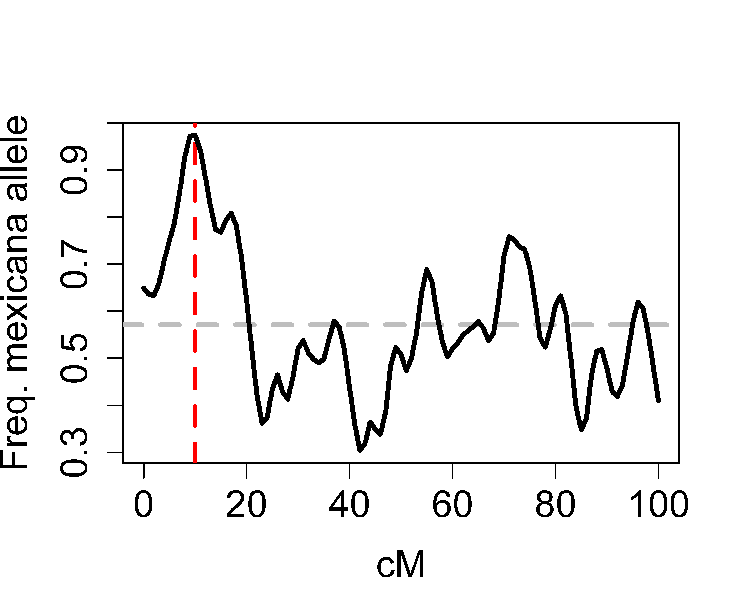
\includegraphics[width=0.4\textwidth]{admix.png}
\label{fig:yaniv}
\end{SCfigure}

%%%%%%%%%%%%%%%%%%%%%%%%%%%%%%%%%%%%%%%%%%%%%%%%%%%%%%%%%%%%%%%%%%%%%%
%AIM 3
%%%%%%%%%%%%%%%%%%%%%%%%%%%%%%%%%%%%%%%%%%%%%%%%%%%%%%%%%%%%%%%%%%%%%%
\section{Functional characterization of adaptive QTL} \label{sec:funchar}

After mapping QTL for highland adaptation (\ref{sec:qtl}) and studying their adaptive significance (\ref{sec:selection}), in this aim we will aim to better understand the functional genetic basis of adaptive regions.  First, we will study the phenotypic effects of alleles at \emph{Inv4m}, an inversion corresponding to a chromosome 4 QTL that has introgressed into highland maize  (\ref{subsec:nils}).  Then, we will use RNA sequencing data to investigate differences in expression, plasticity, and identify potential candidate loci within QTL (\ref{subsec:rnaseq}).

\subsection{Questions}
\begin{itemize}[topsep=0pt,itemsep=-1ex,partopsep=1ex,parsep=1ex]
\item What are the phenotypic consequences of introgressing a single adaptive QTL?
\item What are the functional differences of different alleles of an adaptive QTL?
\item How do maize and teosinte differ in expression response to highland and lowland environments?
\item Can RNA-seq help refine QTL to identify candidate genes?
\end{itemize}

\subsection{Functional evaluation of a Chr 4 QTL} \label{subsec:nils}

In this objective we propose to functionally characterize the genetics of a large \emph{mexicana}-maize introgression block located on chromosomes 4 (Chr4: 169-180Mb). Our previous analysis \citep{Hufford2013} indicates that this region is supported by a robust signature of introgression, shows broad distribution among highland races, and overlaps with a QTL identified in a \emph{parviglumis} x \emph{mexicana} cross  \citep{Lauter2004a} associated with leaf pigmentation and pubescence. Our previous population genetic analysis in teosinte \citep{Pyhajarvi2013}  suggests that the region represents an inversion polymorphism that is under selection along an altitudinal cline, providing the opportunity to characterize the regions as a block through the generation of introgression stocks. % \ref{fig:cline}.  

%\begin{figure}
%  \centering
%   \includegraphics[width=0.7\textwidth]{chr4.png}  \caption{Clinal variation at the Chr4 inversion. Genetic distance (\# of SNPs) from the canonical highland haplotype is plotted against elevation for 20 teosinte populations (shown as different colors).  Low elevation (<1500m) populations lack the inversion completely, while it is fixed in populations abouve 2000m. Data from \citet{Pyhajarvi2013}. } 
%\label{fig:cline} 
%\end{figure}

We will generate heterogeneous inbred families \citep[HIFs;][]{tuinstra1997heterogeneous} from a cross of the landrace Palomero Toluque\~no (PT) and the reference genome inbred B73.  PT is popcorn originating from the highland valleys of central Mexico that is considered basal to the Mexican highland landrace radiation \citep{reif2006grouping}; it also exhibits the highest level of \emph{mexicana} introgression among characterized material \citep{Matsuoka2002}. Furthermore, inspection of the PT genome sequence \citep{Vielle-Calzada2009} shows that PT carries \emph{mexicana} alleles at two SNPs shown previously to exhibit a fixed difference between  \emph{mexicana} and maize \citep{Hufford2013}. We will screen an existing collection of \textasciitilde 150 B73 x PT BC1S3 (three generations of selfing after 1 generation of back-cross) families to identify HIFs segregating for B73 and PT haplotypes using microsatellite makers we have shown distinguish B73 and PT alleles in this region. HIFs will be self-pollinated to generate pairs of near-isogenic lines (NILs) homozygous for the B73 or PT haplotype. While different in the candidate region, NIL pairs will share a common genetic background outside this region, including a sizable (~25\%) contribution of PT, capturing potential epistatic effects important to expression of the candidate phenotype. NILs will be genotyped by GBS  \citep{Elshire 2011, Glaubitz2014} both to confirm the extent of introgression at the Chr4 candidate locus and to characterize this shared background. A total of 6 HIF derived NIL pairs (i.e. 12 lines), will be characterized in our three field sites (Table \ref{tab:locales}) and evaluated for phenotypes described in (Figure \ref{fig:phenos}). In each site, we will plant 3 replicate rows of our NILs and B73 and PT parents. Data will be analyzed broadly as described in \ref{sec:qtlmap}, both treating the introgression region as a single block, or considering individual markers.
f
The expected outcomes of this objective are 1) estimation of the contribution of differences at the Chr4 candidate locus to variation in a number of important phenotypes, 2) determination of the degree of phenotypic plasticity with respect to highland and lowland environments, 3) identification of differences in phenotypic effect among NIL pairs, indicative of background dependent epistatic interaction among genes.

As described above, the Chr4 candidate region is hypothesised to be an inversion polymorphism. While facilitating generation of test materials and assessment of the region as a block, the predicted lack of recombination will hamper downstream efforts to dissect phenotypic effects and fine map the loci involved. Consequently, we will generate a series of NILs by marker-assisted recurrent backcross to B73 using a collection of seven diverse donor varieties: 3 lowland haplotypes represented by the 2 lowland parents of our mapping populations \ref{subsec:qtlmap} and an inbred \emph{parviglumis}; 4 highland haplotypes represented by the 2 highland parents of our mapping populations \ref{subsec:qtlmap} , an inbred \emph{mexicana} and the Palomero Toluque\~no haplotype segregating in our HIFs \ref{subsec:nils}. All 3 highland maize varieties are predicted to carry the \emph{mexicana} inverted haplotype at the Chr4 candidate locus.  Each of these parents either have resequenced genomes \citep{Vielle-Calzada2009, Chia2012a} or will be sequenced as part of this project in \ref{sec:qtl}. It is anticipated that this material will be phenotyped selectively in light of initial results generated in the early part of the project.

{\bf Expected outcomes:} 1) Estimation of functional variation in the Chr4 candidate region among lowland and highland teosinte and landrace maize; 2) Dissection of the highland haplotype on the basis of phenotypic variation among NILs carrying the inverted form; 3) Generation and identification of material suitable for future fine mapping through crossing of genetically/functionally divergent inversions from NILs.   

\subsection{Gene expression} \label{subsec:rnaseq}

We will first assess the effects of high and low elevation environments on genome-wide expression differences to identify genes responsive to these environments.  We will grow the 8 inbred lines which serve as parents of our allelic series analysis in \ref{subsec:nils} in a highland and lowland field site Table \ref{tab:locales}.  From each inbred we will sample leaf and root tissue from three plants at each of two time stages (seedling and flowering adult). Tissue will be flash frozen and sent to UC Davis for extraction and sequencing (multiplexed 12 individuals per lane of an Illumina HiSeq 2500) at the UC Davis Genome Center. Each individual will be barcoded, providing 3 biological replicates for each tissue/time/environment combination. We will assess differences in expression across environments and identify overlap between differentially expressed (DE) genes and QTL from \ref{sec:qtl}, loci showing selection identified in \ref{sec:selection}, and introgressed regions showing phenotypic differences in \ref{subsec:nils}.   These results will help narrow down potential candidate genes in QTL and serve as functional validation of loci showing population genetic evidence of selection in introgressed and admixed populations.  The data will also allow investigation of the relationship between phenotypic plasticity and adaptive change \citep[c.f.][]{Rosas26082013} via comparison of DE genes among environments for a single inbred to differences in DE genes among inbreds to ask whether genes showing a plastic response in unadapted material (lowland landraces, \emph{parviglumis} B73) show constitutive response in adapted lines (\emph{mexicana},highland landraces).  

Our second approach will be a targeted analysis of transcriptomic changes in the Chr4 NIL lines from \ref{subsec:nils}.  Using NILs generated from each of the same 7 inbred donors (alongside an additional replicate of B73), we will evaluate shoot tissues of three plants sampled at seedling and flowering stage for each of the two genotypes (homozygous B73, homozygous donor).  Samples will be extracted and sequenced as described above. These analyses will allow us to refine potential candidate loci within introgressed segments of our NILs, moving us closer to a functional characterization of observed phenotypic differences. Whole-transcriptome comparison to the donor transcriptomes will allow us to differentiate between cis and trans regulation of expression within the Chr4 region, and analysis of co-expression networks \citep[c.f.][]{Swanson-Wagner02072012}, will highlight the effects of introgressed genes on expression patterns in the rest of the genome, enabling us to begin to dissect the genetic pathways involved in adaptive highland traits.

{\bf Expected outcomes:} 1) Identification of candidate genes showing plastic differential expression within lines across environments 2) Identification of candidate genes showing differential expression among lines from different environments 3) Detailed information on the effects of introgressed segments on genome-wide expression. 

\rowcolors{2}{gray!25}{white}
\begin{table}[H]
\begin{center}
\caption{Proposed timeline of activities and responsibilities}\label{tab:timeline}
\begin{tabular}{lccccc}\\\toprule  
    \rowcolor{gray!50}
Year & 2015 & 2016 & 2017 & 2018 & 2019 \\\midrule
Objective \ref{subsec:nils} Functional analyses & -- & RS, AC & AC,JRI & AC,JRI & -- \\\midrule
Objective \ref{subsec:rnaseq} RNA-seq & 2015 & 2016 & 2017 & 2018 & 2019\\\midrule
Objective \ref{subsec:intropopgen} Maize/mexicana introgression & 2015 & 2016 & 2017 & 2018 & 2019 \\\midrule
Objective \ref{subsec:admixmap} Admix mapping & 2015 & 2016 & 2017 & 2018 & 2019 \\\midrule
Objective \ref{subsec:qtlmap} QTL mapping & 2015 & 2016 & 2017 & 2018 & 2019 \\\midrule
Objective \ref{subsec:global} Highland haplotypes & 2015 & 2016 & 2017 & 2018 & 2019 \\\midrule
Objective \ref{subsec:admixpopgen} Admixture population genetics & 2015 & 2016 & 2017 & 2018 & 2019\\ \bottomrule
\end{tabular}
\end{center}
\end{table} 


\required{Broader Impacts}
% As in the project summary, broader impacts must be called out separately 
% in the project description.  You may be able to give more specific
% examples, or discuss how you've previously achieved these impacts.
% It should be similar, but not identical, to the Broader Impacts statement
% in the project summary

%Also mention online presence?  twitter, online dissemination, etc.? slideshare, figshare, preprints, Haldane's sieve?

\subsection*{Exchange Program} 

We propose an international student exchange program between the PIs in the U.S. and Senior Personnel at LANGEBIO in Mexico. Over the course of the grant, we propose to fund 10 graduate or undergraduate students for 3-month research internships in one of the collaborating laboratories. Students involved will participate in research projects directly relating to the research focus of the grant, including developing mapping populations, mapping traits, population genetic analysis, or analysis of next-generation data. The expectation is that such research will often lead to co-authorship on publications. Students will be asked to give two presentations, one to the host lab upon arrival, talking about the lab/university they came from and research there, and another to their host lab detailing their work over the 3-month period.  Each of the PIs will participate, sending students to Mexico and/or accepting students from Mexico for internships. PI Ross-Ibarra will manage the program, as he is fluent in Spanish and has past experience with a similar exchange program (NSF 0922703). Over the last four years, his lab has hosted 6 Mexican students who have worked on various computational aspects of centromere evolution. Two of those students have earned authorship on a paper to be submitted later this year and one has gone on to a PhD program in the U.S.

Our goal is to involve students directly in research while at the same time fostering intercultural exchange and promoting future international research opportunities. It is particularly appropriate for the study of maize, a crop with significant cultural and economic impact in both Mexico and the U.S. Participating Mexican students will learn new analytical methods -- especially computational management of large datasets -- that can be introduced to their respective laboratories and peers. American exchange students will similarly benefit from experience with large field experiments and efforts to functionally characterize individual loci.  The hope is that Mexican undergraduate students involved may be recruited to graduate programs in the U.S., ideally to work in the lab of one of the PIs, and that American undergraduate students will be exposed to international opportunities for research, graduate education, and collaboration.

\subsection*{Phenotyping workshop} %SFG, JRI

The USDA-ARS group in Columbia has developed a streamlined phenotypic data collection system utilizing a handheld barcode device, barcoded plant tags, and barcoded phenotyping tools in order to maximize efficiency.  We will host a phenotyping workshop in Columbia during each year of the grant.  Through this workshop, Dr. Flint-Garcia’s state-of-the-art system will be transferred to other research institutions to aid in large-scale data collection. The phenotyping workshop will include topics on Experimental Design, setting up the FieldBook database, and Data Collection.  Experimental design topics include understanding where variation comes from, how to control for environmental/field variability and experimental error; heritability and repeatability.  The need for consistent data collection and high-throughput will be emphasized.  FieldBook database setup topics include setting up Palm handheld users, locations, traits, projects, assigning plots to projects, assigning traits and measurements to projects,  generating barcoded plant tags, and loading the program and trait groups to the Palm to prepare for data collection.  Topics to be covered in Data Collection include data collection for specific traits related to local adaptation of interest to our group, synchronizing data from the palm with the desktop/laptop database, managing data conflicts between the palm and the database, running reports, and exporting data.  This proposal will provide travel support for instructors.  The workshop will be free but participants will be expected to purchase their own Palm handheld and pay for their own travel.  The workshop will be held each year in late summer so that the participants can gain hands-on experience in data collection in the corn field.

\subsection*{Software} %JRI and GC

A good understanding of population and quantitative genetics is key to a student’s understanding of genetics and evolution, but these subjects are often conceptually quite difficult. An understanding of genetic variation and its phenotypic effects is also an increasingly important part of being an informed citizen, due to the rise of personal genomics and genomic medicine \citep[e.g.][]{redfield2012}. The large amount of population genetic and association data being generated offers a superb chance to motivate these subjects using real data. 
We will develop undergraduate teaching modules in population and quantitative genetics using data from this project. These modules will be tested and integrated into large undergraduate teaching courses (introductory evolutionary biology and genetics) at UC Davis and graduate courses at UC Davis and Iowa State (ecological genomics). We have already begun to develop and distribute some of these resources, e.g. genome-scale demonstrations of Hardy Weinberg Equilibrium (HWE) using  human HapMap data. Such demonstrations underscore the usefulness of basic population genetics in describing real world patterns, and begin to expose students to the wealth of genomics data being collected. 
Other examples will include: using association data from our admixed populations to demonstrate quantitative genetics models; and explaining concepts of genetic and genealogical ancestry using genomic identity by descent.  These modules will be prepared in the open source statistical program R, to ensure that they are easily used, modified, and distributed, and to expose students to programming in biology. The modules will be designed so that they can be tailored for use at a variety of levels from teaching basic concepts to large undergraduate classes to providing the raw data for programming exercises for upper division courses.

The modules will be publicly distributed via Github (see Data Management Plan) in a fully open manner. The use of github will allow others to modify and extend the modules and to share and track these modifications. 

\subsection*{Germplasm resources} %MBH, SFG and RS
%The highland environment remains an important niche for global maize production, in terms of acreage and farmer involvement, if not overall yield. The highland environment presents a number of important abiotic challenges beyond high elevation per se, including periods of drought and cold, and highland adapted material has great potential to provide an important source of stress tolerance; the rapid development and inherent earliness of highland material, for example, may have general application in marginal environments. 

This project will generate multiple germplasm resources.  Seed from the F2 parents will allow additional use of this mapping population to study additional phenotypes of interest (e.g. root morphology and growth).  Seed from our NIL populations will allowing investigation of genome-wide introgressions from a variety of exotic lines.  Such material could be of interest to the Germplasm Enhancement of Maize (http://www.public.iastate.edu/~usda-gem/) project as well as to public and private breeders both in the US and abroad. In Mexico, for example, the highland niche represents a key target market for an emerging private sector of small breeding companies established following deregulation in 1990s. While highland adapted hybrids are available, these are largely derived from lowland sub-tropical material with little or no contribution of the highland landraces and the germplasm developed here could be an important contribution to furthering such programs. Finally, seed from our collections of teosinte will enhance the sampling of these subspecies and provide additional diversity not currently present in germplasm banks.  Seed from our mapping populations will be deposited in the USDA-ARS Maize Stock Center at the University of Illinois, and backups will be kept at Iowa State and Missouri.

%This project will also build further the collaboration between US institutions and LANGEBIO, with a number of Mexican graduate students being directly involved. While Mexican plant science retains a traditionally strength in biochemistry and molecular biology, genetics has been less well represented in recent years. As a consequence, while there is ready access to genomics technologies, the human resources to make the most of the opportunities they present may be lacking. This project provides an excellent opportunity for capacity building in a Mexican institution, with the expectation of a lasting impact through future collaboration.

\required{Results From Prior NSF Support}
% 5 pages or fewer of the 15 pages for entire description document.
% include results from NSF grants received in the past 5 years.
% If supported by more than one grant, choose the most relevant one.

% For each grant, include: 
%	(a) NSF award number, amount, dates of support 
%	(b) The title of this project
%	(c) Publications resulting from this research
%	(d) Summary of the results of the completed work
%	(e) A brief description of data samples available and other research products not described 	      elsewhere
%	(f) For renewed support, a description of the relationship between the completed and 			      proposed work

% Due to space limitations, it is often advisable to use citations rather
% than putting the titles of the publications in the body 
% of this section

\subsection*{Ross-Ibarra, Flint-Garcia: \#1238014: Biology of Rare Alleles in Maize and Its Wild Relatives}
\$13,311,185 (\$2,368,767 to Ross-Ibarra and \$1,206,211 to Flint-Garcia), 05/15/13-04/30/18. PI Edward Buckler, co-PIs J. Doebley, J. Holland, S. Flint-Garcia, Q. Sun, P. Bradbury, S. Mitchell, J. Ross-Ibarra
\par\noindent{\bf Intellectual merit} In the first year we have developed accurate imputation approaches, found evidence for the importance of deleterious variants and non-genic polymorphisms in heterosis and GWAS, documented differences in recombination among the parents of the NAM population, and found population genetic evidence suggesting the importance of demography and purifying selection across the genome.  The grant has produced 18 total publications in its first year (only publications involving PIs Flint-Garcia and Ross-Ibarra are shown below). 
\par\noindent{\bf Broader impacts}  In the first year this project has included 10 postdoctoral and 12 graduate trainees. The GBS workshop and traveling maize exhibit continue to be popular and successful. A new version of the teacher-friendly guide to the evolution of maize has been revised and published online. 
\par\noindent{\bf Publications} \citet{peiffer2013genetic, Romay2013, wills2013many, Mezmouk2014, Peiffer2014, sood2014mining}

\subsection*{Ross-Ibarra: \#0922703: Functional Genomics of Maize Centromeres}
\$5,008,031 (\$754,409 to Ross-Ibarra). 09/01/09-08/31/14. PI Kelly Dawe, co-PIs J. Birchler, J. Jiang, G. Presting, J. Birchler, J. Ross-Ibarra
\par\noindent{\bf Intellectual merit} Centromeres are regions of the genome that organize and regulate chromosome movement, yet the biology of centromeres remains poorly understood. Co-PI Ross-Ibarra's group has focused in particular on the evolutionary genetics of centromeres. This work has demonstrated the remarkable evolutionary lability of centromere tandem repeats, but has shown that there is little evidence in maize for coevolution between centromere sequence and kinetochore proteins. Ongoing work from the Ross-Ibarra lab seeks to characterize kinetochore proteins, assess the phylogenetic evidence for longer-term coevolution, and understand patterns of centromere and genome size variation in natural populations.
\par\noindent{\bf Broader impacts}  Co-PI Ross-Ibarra has established and currently runs an international student exchange program as part of this grant. Data and result of this project have been disseminated via publications and presentations as well as deposited in the maize genetics community database \url{www.maizegdb.org}. Former trainees on the grant include Dr. Matthew Hufford (Co-PI on the current grant). 
\par\noindent{\bf Publications} \citet{Shi2010a, Chia2012a, Fang2012a, Hufford2012, Hufford2012b, Hufford2013, Melters2013a, Kanizay2013, Pyhajarvi2013}

\subsection*{Coop: \#1262645: Collaborative Research: ABI Innovation: Visualization And Statistics For Spatial Population Genomic Analysis. }
\$314,260, with an effective date of 05/01/13. Award Duration: 36 months.
\par\noindent{\bf Intellectual merit} We are developing a set of spatial statistics methods based on Gaussian random fields for the analysis of geographic population genomics data. The first method based on this approach has just been published, allowing a sound statistical framework to distinguish the effects of geographic and ecological distance on genetic isolation. 
\par\noindent{\bf Broader impacts}  The R package of the software has been released online, and has already been used by many molecular ecologists. 
\par\noindent{\bf Publications} \citet{bradburd2013}

\subsection*{Flint-Garcia: \#0820619: Genetic Architecture of Maize and Teosinte}
\$ 9,823,000. 3/1/2009-2/28/2013. PI Edward Buckler, co-PIs J. Doebley, T. Fulton, S. Flint-Garcia, J. Holland, S. Kresovich, M. McMullen, Qi Sun. 
\par\noindent{\bf Intellectual merit}  This project extends over more than a decade, and has pioneered the characterization of population genetic and evolutionary parameters of maize diversity, developed resources to connect this genetic diversity to phenotype through both association and joint linkage-association mapping, conducted fine scale analysis of domestication and agronomic QTL, and recently expanded to whole-genome analysis of diversity, evolution, and phenotype. Overall, the maize diversity project has developed a wide range of approaches and broadened understanding of the maize genome, evolution and adaptation, genetic mapping, and the agricultural improvement of maize. The project successfully released and analyzed the maize Nested Association Mapping (NAM) population, collaborated on making first and second generation haplotype maps for maize, resolved domestication traits, developed a range of novel statistical approaches for association mapping, and dissected complex traits such as flowering time, kernel composition, disease resistance, height, and inflorescence and leaf morphology. 
\par\noindent{\bf Broader impacts} The outreach program included a traveling science museum exhibit on maize diversity, evolution and genetics (seen by at least 300,000 people at five venues to date, including the famous Corn Palace in South Dakota), online Teacher Friendly Guide to the Evolution of Maize, seven Genotyping-By-Sequencing (GBS) workshops (held at primarily at Cornell but has also been held in Kenya), and training of postdocs, graduate students and undergraduates, the vast majority of which have continued in scientific careers.  Former trainees on this grant include Dr. Flint-Garcia  and Dr. Ross-Ibarra  (PIs of the current grant), only their publications are shown below.
\par\noindent{\bf Publications} \citet{Buckler2009, Flint-Garcia2009, Flint-Garcia2009a, Flint-Garcia2009b, Gore2009, McMullen2009, Ross-Ibarra2009a, Bottoms2010, Dubois2010, Zhang2010a, vanheerwaarden2010a, vanheerwaarden2010b, Brown2011b, Morrell2011a, Studer2011b, vanheerwaarden2011a, Tian2011, Chia2012a, Cook2012a, Fang2012a, Hufford2012b, Hung2012, Hung2012a, Romay2013}
